\documentclass[../lecture-notes-148x210.tex]{subfiles}

\begin{document}

\subsection{Basic Definition}

Polynomials \cite[section 17]{Judson_2012} are intensively used in almost all areas of cryptography. In our particular case, polynomials will encode the information about
statements we will need to prove. That being said, let us define what polynomial is.

\begin{definition}
    A \textbf{polynomial} $f(x)$ is a function of the form
    \begin{xequation*}
        p(x) = c_0 + c_1 x + c_2 x^2 + \cdots + c_n x^n = \sum_{k=0}^{n} c_k x^k,
    \end{xequation*}
    where $c_0, c_1, \dots, c_n$ are coefficients of the polynomial.
\end{definition}

Notice that for now we did not specify what are $c_i$'s. We are interested in the case where $c_i \in \mathbb{F}$, where $\mathbb{F}$ is a field. 

\begin{definition}
    A set of polynomials depending on $x$ with coefficients in a field $\mathbb{F}$ is denoted as $\mathbb{F}[x]$, that is
    \begin{xequation}
        \mathbb{F}[x] = \left\{p(x) = \sum_{k=0}^{n} c_k x^k: c_k \in \mathbb{F}, \; k = 0,\dots,n\right\}.
    \end{xequation}
\end{definition}

\vspace{-4mm}

\begin{definition}
    Evaluation of a polynomial $p(x) \in \mathbb{F}[x]$ at point $x_0 \in \mathbb{F}$ is simply finding the value of $p(x_0) \in \mathbb{F}$.
\end{definition}

\vspace{-4mm}

\begin{example}
    Consider the finite field $\mathbb{F}_3$. Then, some examples of polynomials from $\mathbb{F}_3[x]$ are listed below:
    \begin{enumerate}
        \item $p(x) = 1 + x + 2x^2$.
        \item $q(x) = 1 + x^2 + x^3$.
        \item $r(x) = 2x^3$.
    \end{enumerate}

   If we were to evaluate these polynomials at $1 \in \mathbb{F}_3$, we would get:
    \begin{enumerate}
        \item $p(1) = 1 + 1 + 2 \cdot 1 \; \text{mod} \; 3 = 1$.
        \item $q(1) = 1 + 1 + 1 \; \text{mod} \; 3 = 0$.
        \item $r(1) = 2 \cdot 1 = 2$.
    \end{enumerate}
\end{example}

\vspace{-4mm}

\begin{definition}
    The \textbf{degree} of a polynomial $p(x) = c_0+c_1x+c_2x^2+\dots$ is the largest $k \in \mathbb{Z}_{\geq 0}$ such that $c_k \neq 0$. We denote the degree of a polynomial as $\deg p$. We also denote by $\mathbb{F}^{(\leq m)}[x]$ a set of polynomials of degree at most $m$.
\end{definition}

\begin{example}
    The degree of the polynomial $p(x) = 1 + 2x + 3x^2$ is $2$, so $p(x) \in
    \mathbb{F}_5^{(\leq 2)}[x]$.
\end{example}

\begin{theorem}
    For any two polynomials $p,q \in \mathbb{F}[x]$ and $n = \deg p, m = \deg q$, the following two statements are true:
    \begin{enumerate}
        \item $\deg (pq) = n + m$.
        \item $\deg (p + q) = \max\{n,m\}$ if $n \neq m$ and $\deg (p+q) \leq m$ for $m=n$.
    \end{enumerate}
\end{theorem}

\subsection{Roots and divisibility}

\begin{definition}
    Let $p(x) \in \mathbb{F}[x]$ be a polynomial of degree $\deg p \geq 1$. A field element $x_0 \in \mathbb{F}$ is called a root of $p(x)$ if $p(x_0) = 0$.
\end{definition}

\vspace{-4mm}

\begin{example}
    Consider the polynomial $p(x) = 1 + x + x^2 \in \mathbb{F}_3[x]$. Then, $x_0=1$ is a root of $p(x)$ since $p(x_0) = 1 + 1 + 1 \; \text{mod} \; 3 = 0$.
\end{example}

One of the fundamental theorems of polynomials is following.

\begin{theorem}
    Let $p(x) \in \mathbb{F}[x], \deg p \geq 1$. Then, $x_0 \in \mathbb{F}$ is a root of $p(x)$ if and only if there exists a polynomial $q(x)$ (with $\deg q = n-1$) such that
    \begin{xequation}
        p(x) = (x-x_0)q(x)
    \end{xequation}
\end{theorem}

\begin{example}
    Note that $x_0=1$ is a root of $p(x) = x^2+2$. Indeed, we can write $p(x) = (x-1)(x-2)$, so here $q(x) = x-2$.
\end{example}

Also, this might not be obvious, but we can also divide polynomials in the same way as we divide integers. The result of division is not always a polynomial, so we also get a remainder.

\begin{theorem}
    Given $f,g \in \mathbb{F}[x]$ with $g \neq 0$, there are unique polynomials $p,q \in \mathbb{F}[x]$ such that 
    \begin{xequation}
        f = q \cdot g + r, \; 0 \leq \deg r < \deg g
    \end{xequation}
\end{theorem}

\begin{example}
    Consider $f(x) = x^3+2$ and $g(x) = x+1$ over $\mathbb{R}$. Then, we can write $f(x) = (x^2-x+1)g(x) + 1$, so the remainder of the division is $1$. Typically, we denote this as:
    \begin{xequation*}
        f \, \text{div} \, g = x^2-x+1, \quad f \, \text{mod} \, g = 1.
    \end{xequation*}

    The notation is pretty similar to one used in integer division.
\end{example}

Similarly, one can define $\text{gcd}$, $\text{lcm}$, and other number field theory operations for polynomials. However, we will not go into details here, besides mentioning the divisibility.

\begin{definition}
    A polynomial $f(x) \in \mathbb{F}[x]$ is called \textbf{divisible} by $g(x) \in \mathbb{F}[x]$ (or, $g$ \textbf{divides} $f$, written as $g \mid f$) if there exists a polynomial $h(x) \in \mathbb{F}[x]$ such that $f=gh$.
\end{definition}

\begin{theorem}
    If $x_0 \in \mathbb{F}$ is a root of $p(x) \in \mathbb{F}[x]$, then $(x-x_0) \mid p(x)$.
\end{theorem}

\begin{definition}
    A polynomial $f(x) \in \mathbb{F}[x]$ is said to be \textbf{irreducible} in $\mathbb{F}$ if there are no polynomials $g,h \in \mathbb{F}[x]$ both of degree more than $1$ such that $f = gh$.
\end{definition}

\begin{example}
    A polynomial $f(x) = x^2+16$ is irreducible in $\mathbb{R}$. In turn, $f(x) = x^2-2$ is not irreducible since $f(x) = (x-\sqrt{2})(x+\sqrt{2})$. 
\end{example}

\begin{example}
    There are no polynomials over complex numbers $\mathbb{C}$ with degree more than $2$ that are irreducible. This follows from the \textit{fundamental theorem of algebra}.
\end{example}

\subsection{Interpolation}

Now, let us ask the question: what defines the polynomial? Well, given expression $p(x) = \sum_{k=0}^n c_kx^k$ one can easily say: ``hey, I need to know the coefficients $\{c_k\}_{k=0}^n$''.

Indeed, each polynomial of degree $n$ is uniquely determined by the vector of its coefficients $(c_0,c_1,\dots,c_n) \in \mathbb{F}^n$. However, that is not the only way to define a polynomial.

Suppose I tell you that $p(x) = ax + b$ -- just a simple linear function over $\mathbb{R}$. Suppose I tell you that $p(x)$ intercepts $(0,0)$ and $(1,2)$. Then, you can easily say that $p(x) = 2x$. 

The more general question is: suppose $\deg p = n$, how many points do I need to define the polynomial $p(x)$ uniquely? The answer is $n+1$ distinct points. This is the idea behind the interpolation:
the polynomial is uniquely defined by $n+1$ distinct points on the plane. An example is depicted 
in Figure~\ref{fig:interpolation}. Now, let us see how we can interpolate the polynomial practically.

\begin{figure}[H]
    \centering
    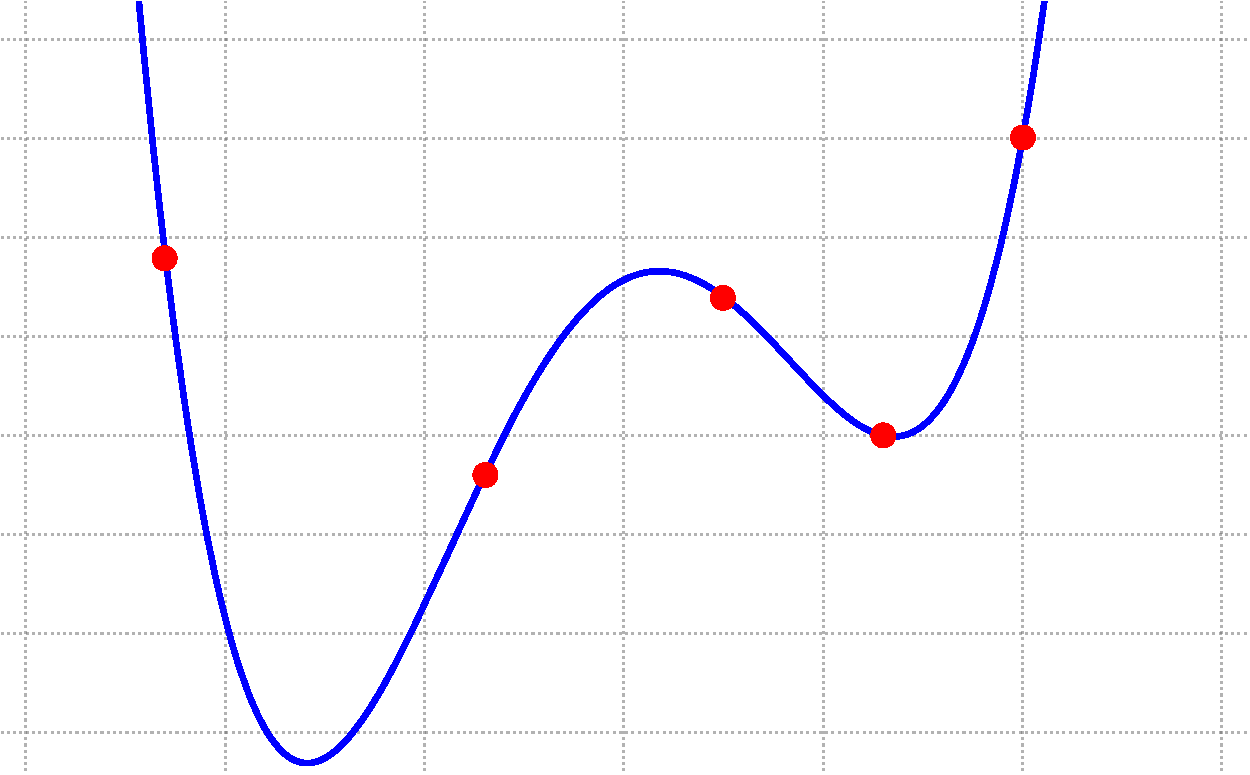
\includegraphics[width=0.8\textwidth]{images/lecture_1/interpolation.pdf}
    \caption{$5$ points on the plane uniquely define the polynomial of degree $4$.}
    \label{fig:interpolation}
\end{figure}

\begin{theorem}
    Given a set of points $\{(x_0,y_0),(x_1,y_1),\dots,(x_n,y_n)\} \subset
    \mathbb{F} \times \mathbb{F}$, there is a unique polynomial $L(x)$ of degree
    $n$ such that $L(x_i) = y_i$ for all $i=0,\dots,n$. This polynomial is
    called the \textbf{Lagrange interpolation polynomial} \cite{Saniee_2007_LagrangeInterpolation} and can be found
    through the following formula:
    \begin{xequation}
        L(x) = \sum_{i=0}^{n} y_i \ell_i(x), \quad \ell_i(x) = \prod_{j=0, j \neq i}^{n} \frac{x-x_j}{x_i-x_j}.
    \end{xequation}
\end{theorem}

\begin{lemma}
    The polynomials $\{\ell_i\}_{i=1}^n$, in fact, have quite an interesting property:
    \begin{xequation*}
        \ell_i(x_j) = \delta_{ij} = \begin{cases}
            1, & i = j \\ 0, & i \neq j
        \end{cases},
    \end{xequation*}
    where $\delta_{ij}$ is the Kronecker delta. Moreover, $\{\ell_i\}_{i=1}^n$ form a basis of $\mathbb{F}^{(\leq n)}[x]$: for any polynomial $p(x) \in \mathbb{F}^{(\leq n)}[x]$ there exist unique coefficients $\alpha_0,\dots,\alpha_n \in \mathbb{F}$ such that
    \begin{xequation}
        p(x) = \sum_{i=0}^{n} \alpha_i \ell_i(x).
    \end{xequation}
\end{lemma}

\begin{example}
    Suppose we have points $(0,1)$ and $(1,2)$. Then, the Lagrange interpolation polynomial is
    \begin{equation*}
        L(x) = 1 \cdot \frac{x-1}{0-1} + 2 \cdot \frac{x-0}{1-0} = (-1) \cdot (x-1) + 2 \cdot x = x + 1
    \end{equation*}
\end{example}

\subsection{Schwartz-Zippel Lemma}

Schwartz-Zippel Lemma is central for most modern zero-knowledge protocols. Its
simple interpretation is the following: if we want to check whether two
polynomials are equal, we can do it by checking whether they are equal at a
random point. The probability of two different polynomials being equal at a
random point is very low for sufficiently large finite fields $\mathbb{F}$.
However, let us formulate the lemma more rigorously. Let us start with the
single-variable case, which is easiest to understand.

\vspace{-0.6mm}

\begin{lemma}[Single Variable Schwartz-Zippel Lemma]\label{lemma:one-sz} Let
    $\mathbb{F}$ be a finite field and let $f \in \mathbb{F}[x]$ be a
    polynomial. Then,
    \begin{xequation}
        \underset{x \xleftarrow{R} \mathbb{F}}{\text{Pr}}
        [f(x) = 0] \leq \frac{\deg f}{\left|\mathbb{F}\right|}.
    \end{xequation}
\end{lemma}

\vspace{-0.6mm}

\textbf{Proof Idea.} The proof is quite simple. The polynomial of degree up to
$n:=\deg f$ can have up to $n$ roots. Therefore, when we pick the point $x$
uniformly at random from the field $\mathbb{F}$, there is at most $n/|\mathbb{F}|$
chance to pick the root of the polynomial.

However, the lemma can be generalized to the multi-variable case, which is more
difficult to prove. The generalization is as follows.

\vspace{-0.6mm}

\begin{lemma}[Multivariable Schwartz-Zippel \cite{Oveis_Gharan_2017_Lecture7}] \label{lemma:sz}
    Let $\mathbb{F}$ be a finite field and $\mathbb{S} \subseteq \mathbb{F}^n$ be a finite $n$-dimensional subspace.
    Let $f: \mathbb{S} \to \mathbb{F}$ be a polynomial in $n$ variables. Then,
    
    \vspace{-1.1mm}
    
    \begin{xequation}
        \underset{\mathbf{x} \xleftarrow{R} \mathbb{S}}{\text{Pr}}
        [f(\mathbf{x}) = 0] \leq \frac{\deg f}{\left|\mathbb{S}\right|}.
    \end{xequation}
\end{lemma}

\vspace{-4.1mm}

\begin{example}
Suppose we are working over the Mersenne prime field of order $p=2^{31}-1$ with
a polynomial $f(x_1,x_2) = x_1^{50} + 3x_1x_2 + x_2^5$. If we pick $(x_1,x_2)$
at random from $\mathbb{F}_p^2$, the probability of $f(x_1,x_2) = 0$ is at most
$50/(2^{31}-1)$, providing approximately 25 bits of security.
\end{example}

\subsection{Some Fun: Shamir's Secret Sharing}

Shamir's Secret Sharing, also known as $(t,n)$-threshold scheme, is one of the protocols exploiting Lagrange Interpolation. 

But first, let us define what secret sharing is. Suppose we have a secret data $\alpha$, which is represented as an element from some finite set $F$. We divide this secret into $n$ pieces $\alpha_1,\dots,\alpha_n \in F$ in such a way:
\begin{enumerate}
    \item Knowledge of any $t$ shares can reconstruct the secret $\alpha$.
    \item Knowledge of any number of shares below $t$ cannot be used to reconstruct the secret $\alpha$.
\end{enumerate}

Now, let us define the sharing scheme.

\begin{definition}
    \textbf{Secret Sharing} scheme is a pair of efficient algorithms $(\mathsf{Gen}, \mathsf{Comb})$ which work as follows:
    \begin{itemize}
        \item $\mathsf{Gen}(\alpha, t, n)$: probabilistic sharing algorithm that yields $n$ shards $(\alpha_1,\dots,\alpha_t)$ for which $t$ shards are needed to reconstruct the secret~$\alpha$.
        \item $\mathsf{Comb}(\mathcal{I}, \{\alpha_i\}_{i \in \mathcal{I}})$: deterministic reconstruction algorithm that reconstructs the secret $\alpha$ from the shards $\mathcal{I} \subset \{1,\dots,n\}$ of size~$t$.
    \end{itemize}

    Here, we require the \textbf{correctness}: for every $\alpha \in F$, for every possible output $(\alpha_1,\dots,\alpha_n) \gets \mathsf{Gen}(\alpha, t, n)$, and any $t$-size subset $\mathcal{I}$ of $\{1,\dots,n\}$ we have
    \begin{xequation}
        \mathsf{Comb}(\mathcal{I}, \{\alpha_i\}_{i \in \mathcal{I}}) = \alpha.
    \end{xequation}
\end{definition}

Now, Shamir's protocol is one of the most famous secret sharing schemes. It works as follows: our finite set is $\mathbb{F}_q$ for some large prime $q$. Then, algorithms in the protocol are defined as follows:
\begin{itemize}
    \item $\mathsf{Gen}(\alpha, k, n)$: choose random $k_1,\dots,k_{t-1}
    \xleftarrow[]{R} \mathbb{F}_q$ and define polynomial $\omega(x) := \alpha +
    \sum_{j=1}^{t-1}k_jx^j \in \mathbb{F}_q^{\leq (t-1)}[x]$. Then, compute
    $\alpha_i \gets \omega(i) \in \mathbb{F}_q$ for each $i$ and return
    $(\alpha_1,\dots,\alpha_n)$.
    \item $\mathsf{Comb}(\mathcal{I}, \{\alpha_i\}_{i \in \mathcal{I}})$: reconstruct the polynomial $\omega(x)$ using Lagrange interpolation and return $\omega(0) = \alpha$.
\end{itemize}

The combination function is possible since, having $t$ points $\{i,\alpha_i\}_{i
\in \mathcal{I}}$ with $\omega(i) = \alpha_i$, we can fully reconstruct the
polynomial $\omega(x)$ and then evaluate it at $0$ to get $\alpha$. Instead,
suppose we have only $t-1$ (or less) pairs $\{i,\alpha_i\}_{i \in \mathcal{I}}$.
Then, there are many polynomials $\omega(x)$ that pass through these points (in
fact, if we were in the field of real numbers, this number would be infinite),
and thus the secret $\alpha$ is not uniquely determined. The intuition behind
Shamir's Secret Sharing protocol is illustrated in Figure~\ref{fig:shamir}: for
$t=3$, having only two \textcolor{blue}{blue} points, we cannot reconstruct the
polynomial, while knowing the third \textcolor{red}{red} point allows us to
uniquely determine the polynomial and thus get value at $0$.

\vspace{-2mm}

\begin{figure}[H]
    \centering
    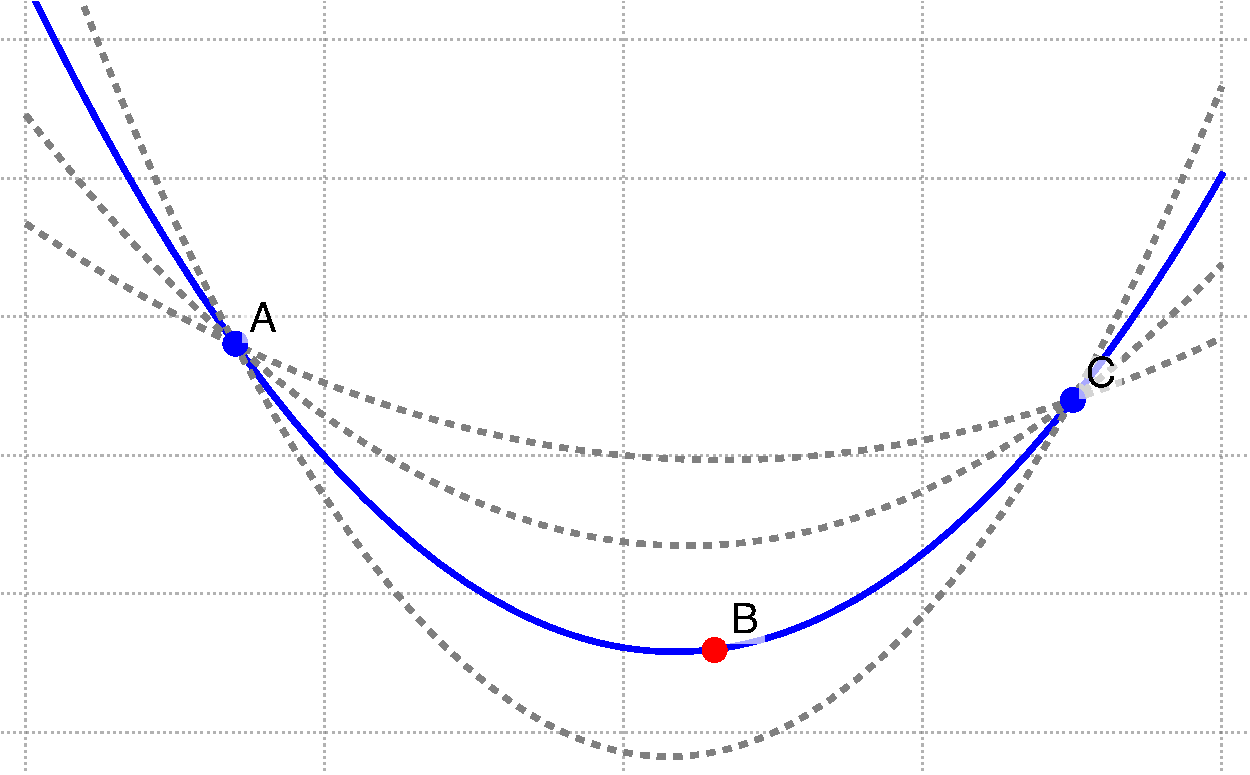
\includegraphics[width=0.5\textwidth]{images/lecture_1/shamir_demo.pdf}
    \caption{Illustration of Shamir's Secret Sharing}
    \label{fig:shamir}
\end{figure}

\subsection{Exercises}

\begin{xexercise}
    {Exercise 1.}
    {
        Suppose for three polynomials $p,q,r \in \mathbb{F}[x]$ we have $\deg p = 3, \deg q = 4, \deg r = 5$. 
        Which of the following is true for $n := \deg \{(p-q)r\}$?
        \vspace{-3.5mm}
    }
    {2}
    {
        \item $n = 9$.
        \item $n$ might be less than $9$.
        \item $n = 20$.
        \item $n$ is less than $\deg \{qr\}$. 
    }
\end{xexercise}

\begin{xexercise}
    {Exercise 2.}
    {
        Define the polynomial over $\mathbb{F}_5$: $f(x) := 4x^2 + 2$. Which of the following is the root of $f(x)$?
    }
    {2}
    {
        \item $2$
        \item $3$
        \item $4$
        \item $f$ has no roots.
    }
\end{xexercise}

\begin{xexercise}
    {Exercise 3.}
    {
        Quadratic polynomial $p(x) = ax^2+bx+c \in \mathbb{R}[x]$ has zeros at $1$ and $2$ and $p(0) = 2$. 
        Find the value of $a+b+c$.
    }
    {2}
    {
        \item $0$
        \item $-1$
        \item $1$
        \item Not enough information is provided.
    }
\end{xexercise}

\begin{xexercise}
    {Exercise 4*.}
    {
        Consider two polynomials: 
        \begin{xequation}
            P_n(x) = x^{2n} + x^n -2, \quad Q(x) = x^2 + 1
        \end{xequation}
        For which values of $n$ does polynomial $Q(x)$ divides $P_n(x)$
    }
    {1}
    {
        \item For all even $n$.
        \item For all odd $n$.
        \item For all $n$ which are divisible by 4.
        \item Just for $n = 4$.
        \item It does not work for any natural number $n$.
    }
\end{xexercise}

\begin{xexercise}
    {Exercise 5.} { Suppose $f \in \mathbb{F}_p[x]$ is a $d$-degree polynomial
    with $d$ \textbf{distinct} roots in $\mathbb{F}_p$. Suppose Alice wants to
    fool Bob by claiming that $f$ is not a zero polynomial. The protocol
    consists of $n$ rounds, where on each round Bob samples the random scalar
    $\tau \xleftarrow{R} \mathbb{F}_p$ and checks the value of $f(\tau)$. What
    is the probability that Alice successfully fools Bob during the protocol?}
    {2} {
        \item Exactly $(d/p)^n$
        \item Strictly less than $(d/p)^n$
        \item Exactly $nd/p$.
        \item Strictly less than $d/np$.
    }
\end{xexercise}

\begin{xexercise}
    {Exercise 6.} { Suppose $f \in \mathbb{F}_p[x_1,\dots,x_n]$ is an
    $n$-variable polynomial. Carol randomly samples the point $\mathbf{x}
    \xleftarrow{R} \mathbb{S}$ where $\mathbb{S} \subseteq \mathbb{F}_p^n$ is a
    set of points $(x_1,\dots,x_n)$ such that $\sum_{i=1}^n x_i=1$ over
    $\mathbb{F}_p$. According to the Schwartz-Zippel Lemma, what is the tightest
    upper bound for $\Pr[f(\mathbf{x})=0]$ among specified below?}
    {1} {
        \item $\deg f/p^n$
        \item $\deg f/p^{n-1}$
        \item $\deg f/p^{n-2}$
        \item $\deg f/p$
    }
\end{xexercise}

\end{document}
